\documentclass[a4paper,10pt]{article}
\usepackage[utf8]{inputenc}
\usepackage{graphicx}
\usepackage{url}

\begin{document}

\section{Graphic User Interface}
Evacuation Simulator graphic user interface is built using Java Swing. The benefits of using Swing are firstly it provides a rich set of 
components based on 100\% Java which can be run across all platforms~\cite{jGuru}, secondly Swing components can change their appearance based on the current 
"look and feel" library that's being used(user can use the same look and feel as the platform he is on, or use a different look and feel)~\cite{jGuru} and 
finally and the most importantly, Swing components follow the Model-View-Controller paradigm (MVC), and thus can provide a much more flexible UI~\cite{mvc}.
With these advantages, the system is organised into
\begin{itemize}
 \item Model - represents Data Structures generating path for population to evacuate
 \item View - represents the content of model which is jMonkey and Swing
 \item Controller - represents algorithms when user triggers some action
\end{itemize}
jMonkeyEngine provides a drag and drop features. These save a lot of time since user does not have to do hard coding.
The interface contains many components and this section will give a brief overview. Figure 1 shows the screenshot of Evacuation Simulator interface.
\\
\begin{center}
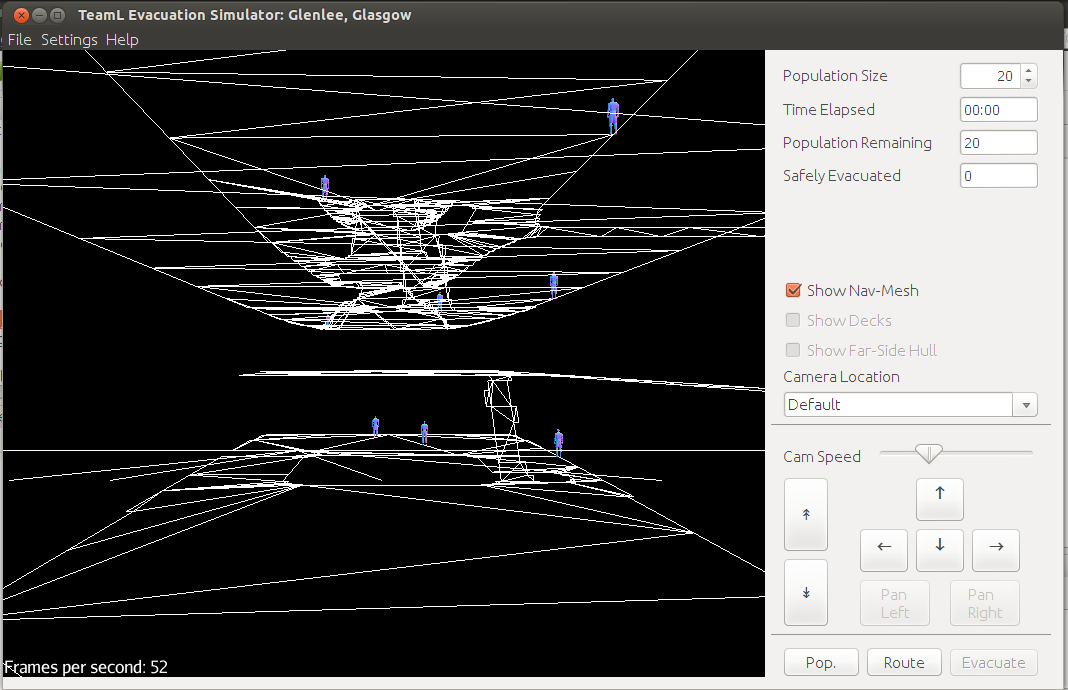
\includegraphics[scale=0.3]{gui.png}
\\Figure 1: Evacuation Simulator Interface
\end{center}
There is a series of buttons categorised by their use. First of all, game play control buttons consisting of populate, evacuate, and 
route generating button provide user with the evacuation control. User can play or pause the evacuation by clicking the evacuate button and resume button 
as they are the same button. There are navigation buttons above the control buttons which user can navigate through the environment. 
Navigation includes moving vertically and horizontally across X, Y and Z axis. To make the evacuation simulator easy to use and faster, 
features to change the camera speed by sliding the camera speed slider which affects the speed of the simulator and to conveniently 
change the camera position to the exit routes by selecting the camera location drop down box are included. Occassionally, it is more apparent to include or not include 
ship frame, ship decks and far-side hull because environment can be seen clearly. This can be done by checking or unchecking the checkboxes provided.
\\

The top-right corner is a widget showing system status which includes population size, time elapsed, population remaining and population safely evacuated.
These features are grouped together in one place to make it easy for user to view system status.
\\

To help user with usability, there are three menubars file, setting and help menubars. File menubar allows user to import 
model in case user wishes to simulate different model in the future.
\\

In terms of settings, our evacuation simulator provides a user with a number of configurations according to user's preference. Initially, when user 
starts the program the settings are set to default values. However, he or she may want to categorise a number of people in the evacuation simulator. For example,
he wants to set a group called Teenager (10 people), Adult (20 people) and Athlete (4 people) with specific properties. This can be done in advanced 
settings. The settings can be saved for future use as well.
Finally, help menubar item provides the user with the guides about how to use and purpose of the program. 
Due to a large space needed to include these features in one window frame, they will be shown in other dialogs.

\begin{center}
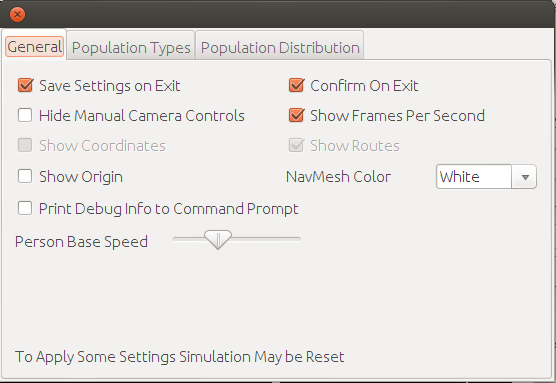
\includegraphics[scale=0.5]{generalsettings.png}
\\Figure 2: General Settings Dialog
\end{center}
General Settings: provides a user with a number of checkboxes, a combobox and a slider to configure system general settings such as changing 
route color, or automatically saving configurations after exit.
\\
\begin{center}
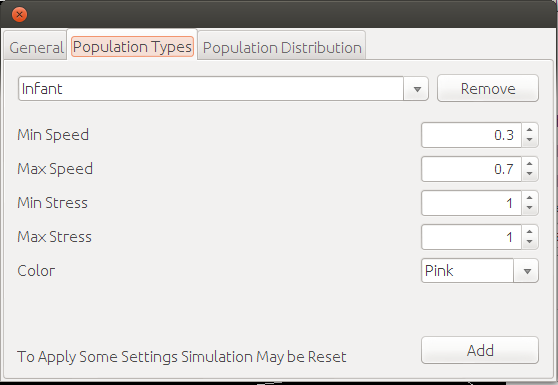
\includegraphics[scale=0.5]{populationSettingsGUI.png}
\\Figure 3: Population Settings Dialog
\end{center}

Population Settings: provides a user with buttons, combobox and spinboxes to add, or remove category of evacuee and modify properties of each category
such as speed, initial stress, personal space(metre) and social priority. Figure 2 shows the screenshot of population settings dialog.

\begin{center}
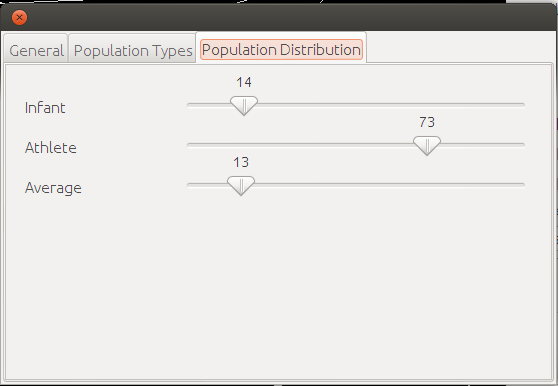
\includegraphics[scale=0.5]{distributionSettingsGUI.png}
\\Figure 3: Distribution Settings Dialog
\end{center}

Distribution Settings: provides a user with a table of categories and their values. User can modify these values. 
Figure 4 shows the screenshot of distribution settings dialog.
\\

To be specific in advanced settings option, advanced settings dialog comprises three different tabs: general settings, population settings 
and distribution settings. Screenshots above show the interfaces of these tabs. \\

\bibliographystyle{unsrt}

\bibliography{individual_ref}

\end{document}









